\begin{figure}
    \begin{center}
    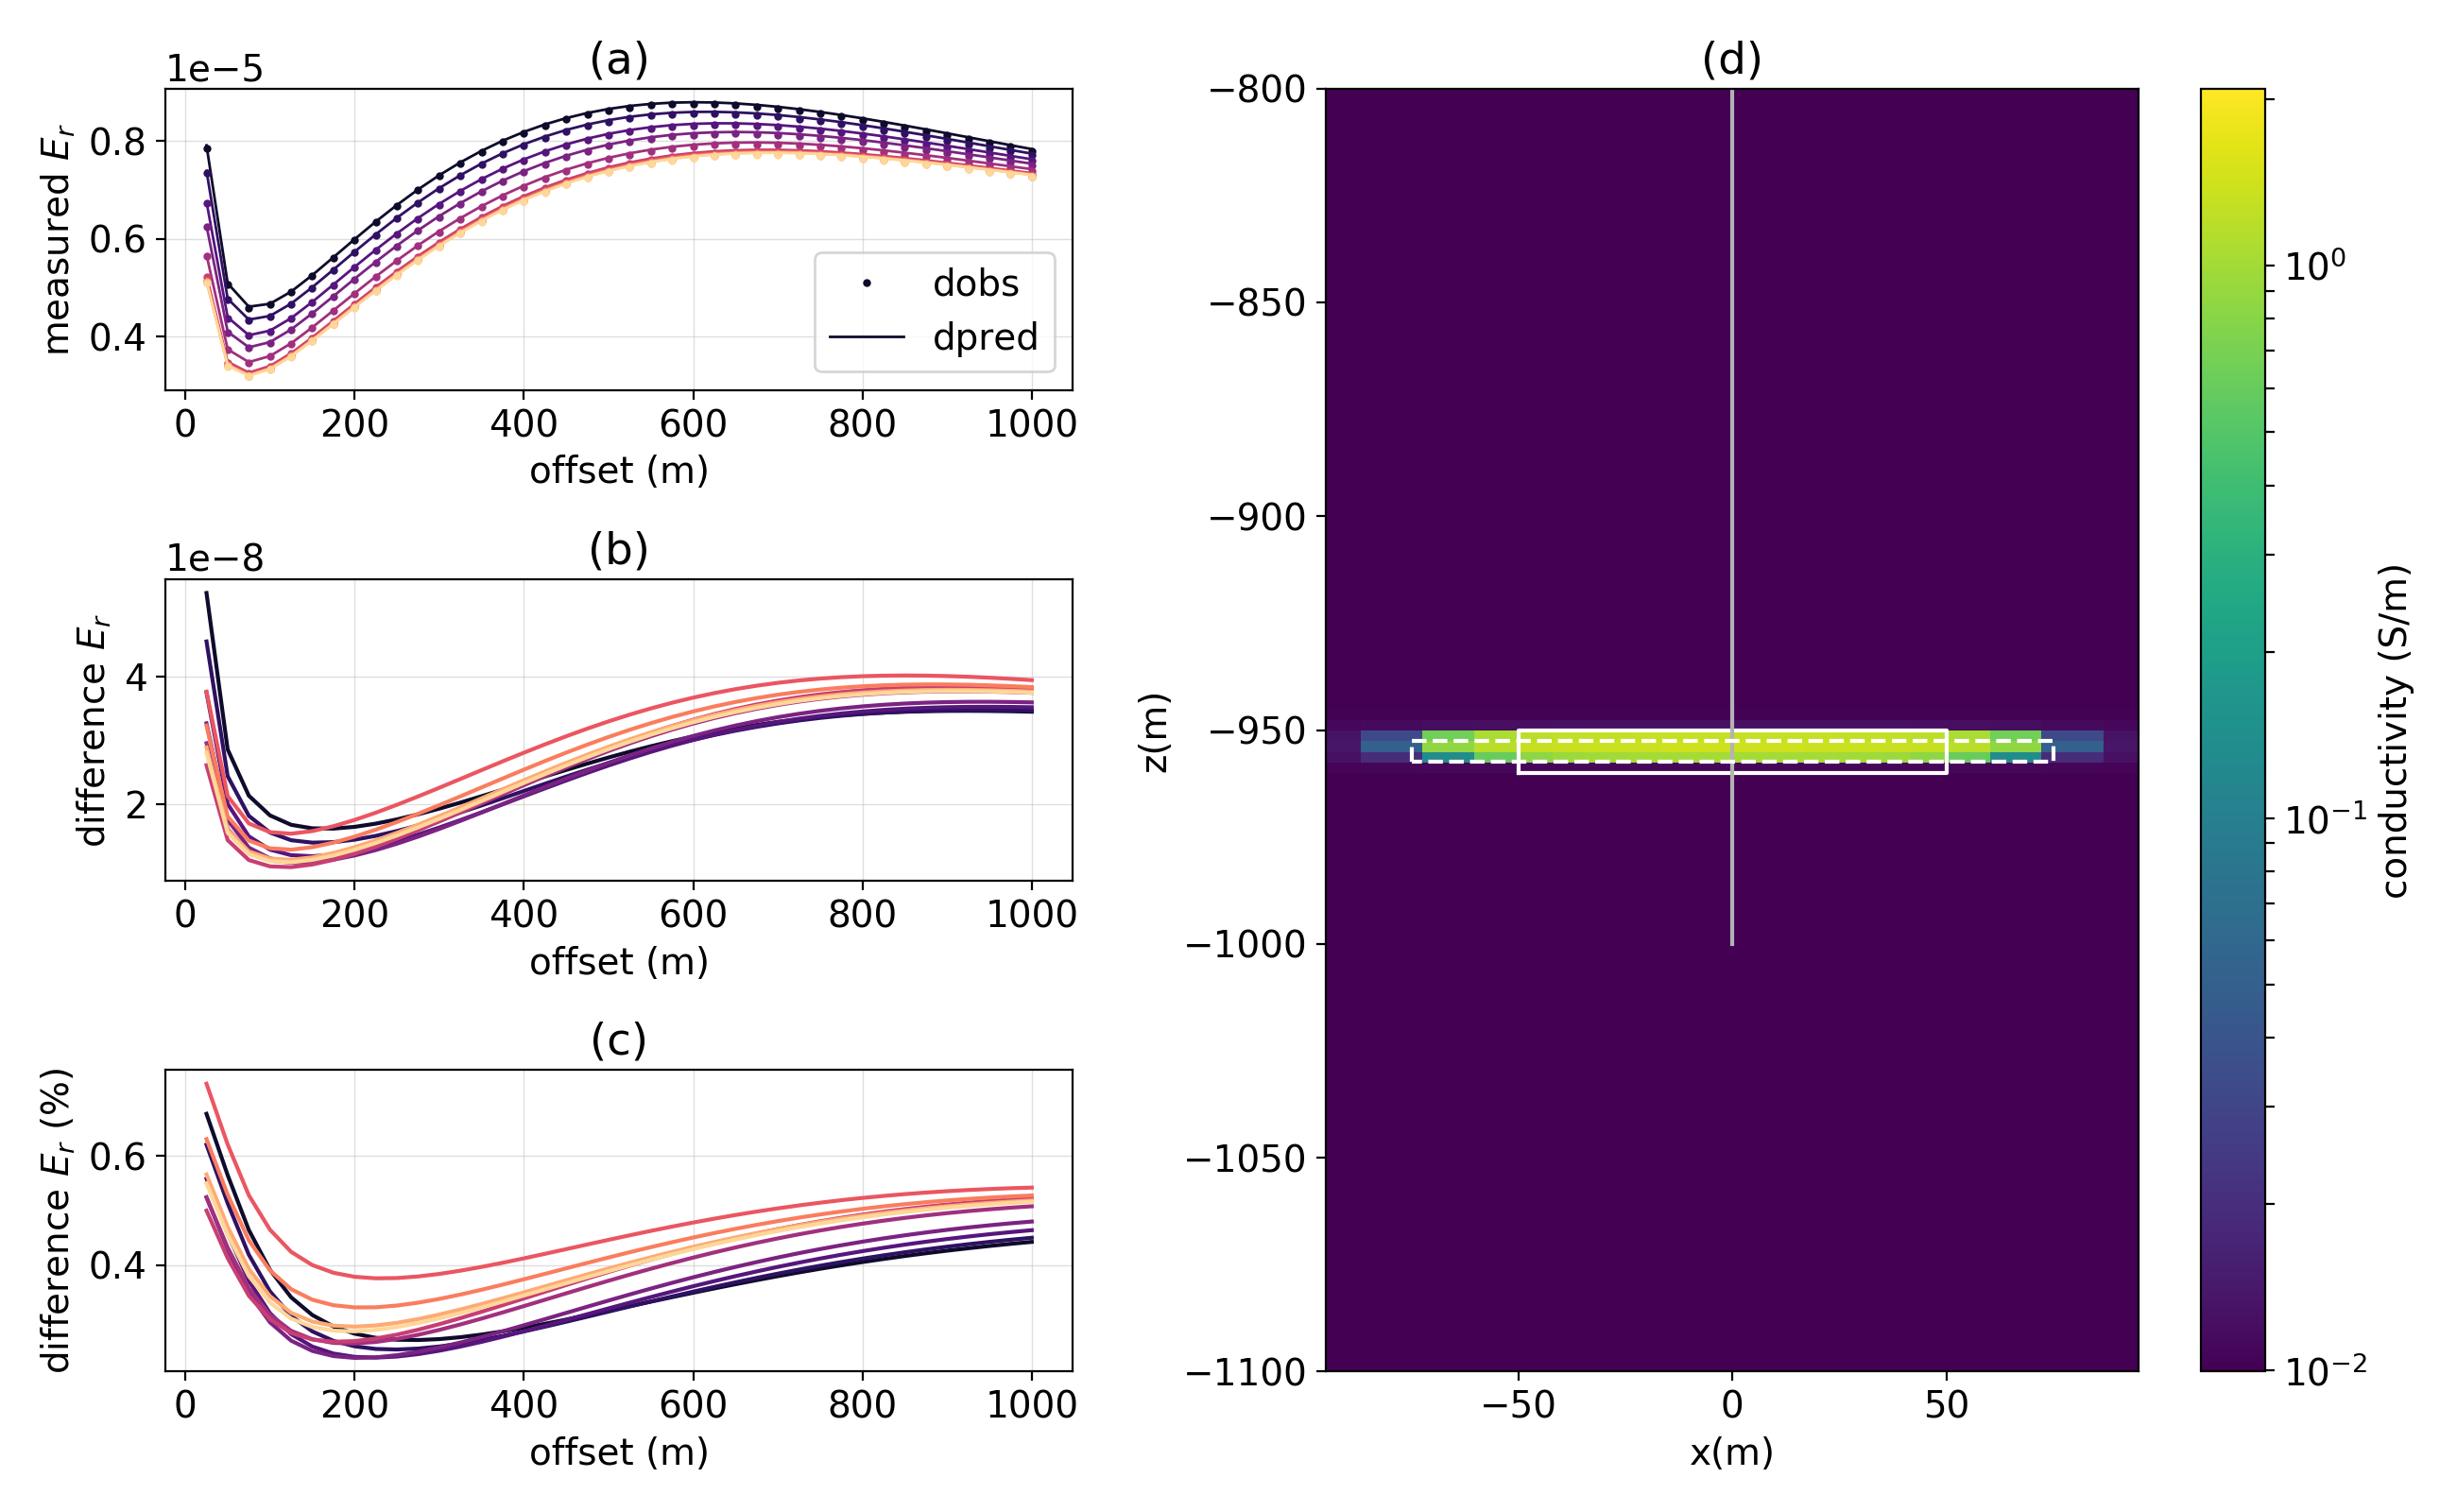
\includegraphics[width=0.8\textwidth]{figures/inversion/parametric_voxel2_large_r.png}
    \end{center}
\caption{
    Parametric inversion result where the center of the target is fixed at a depth
    of 955m. The starting model has a thickness of 5m and a radius of 75m. The initial background
    conductivity is $10^{-2}$ S/m and the initial conductivity of the target is $3\times10^{-2}$ S/m.
    The geometry of the starting model is shown by the white dashed-lines and the
    true model is shown by the solid white outline. The inversion reached a $\chi$-factor $<$ 0.05
    and took 6 iterations.
}
\label{fig:parametric_voxel2_large_r}
\end{figure}
